%% Reduced-Order Forecasting of Particle-Laden Flow Evolution
%% Skeleton for a short (4-6 page) two-column paper. Build with latexmk -pdf main.tex
%% or press F5 in TeXstudio. Figures are pulled from ../docs/figures.

\documentclass[conference,a4paper]{IEEEtran}

\usepackage{graphicx}
\usepackage{amsmath,amssymb}
\usepackage{booktabs}
\usepackage{siunitx}
\usepackage[hidelinks]{hyperref}
\usepackage{cite}

\graphicspath{{../docs/figures/}}

\begin{document}

\title{Reduced-Order Forecasting of Particle-Laden Flow Evolution}

\author{\IEEEauthorblockN{Thomas Bainbridge}
\IEEEauthorblockA{% affiliation
Cranfield University \\
\texttt{tb.engineering.uk@gmail.com}}}

\maketitle

\begin{abstract}
% One paragraph: the problem, what was built, what was compared, the headline
% finding, and the honest caveat. Write last.
\end{abstract}

\begin{IEEEkeywords}
reduced-order modelling, inertial particles, preferential concentration,
dynamic mode decomposition, latent forecasting
\end{IEEEkeywords}

\section{Introduction}
% Why particle-laden flow is expensive to simulate; why the concentration field
% is the quantity of interest; what question this study asks.

\section{Physical Model and Dataset}

\subsection{Carrier Flow}
% Taylor-Green vortex; the multi-mode Fourier option; divergence-free by
% construction.
\begin{equation}
  \mathbf{u}(x,y,t) = A(t)\begin{pmatrix}\sin x\cos y\\ -\cos x\sin y\end{pmatrix},
  \qquad \nabla\cdot\mathbf{u} = 0 .
  \label{eq:carrier}
\end{equation}

\subsection{Inertial Particles}
% Linear Stokes drag, RK4 integration, the Stokes number as the only parameter.
\begin{equation}
  \frac{d\mathbf{v}_p}{dt} = \frac{\mathbf{u}(\mathbf{x}_p,t) - \mathbf{v}_p}{\tau_p},
  \qquad \mathrm{St} = \tau_p/\tau_f .
  \label{eq:particles}
\end{equation}

\subsection{Concentration Fields}
% Lagrangian to Eulerian binning; the sweep (4 Stokes numbers x 5 seeds, 201
% snapshots); the raw vs Gaussian-KDE-smoothed variants.

\begin{figure}[t]
  \centering
  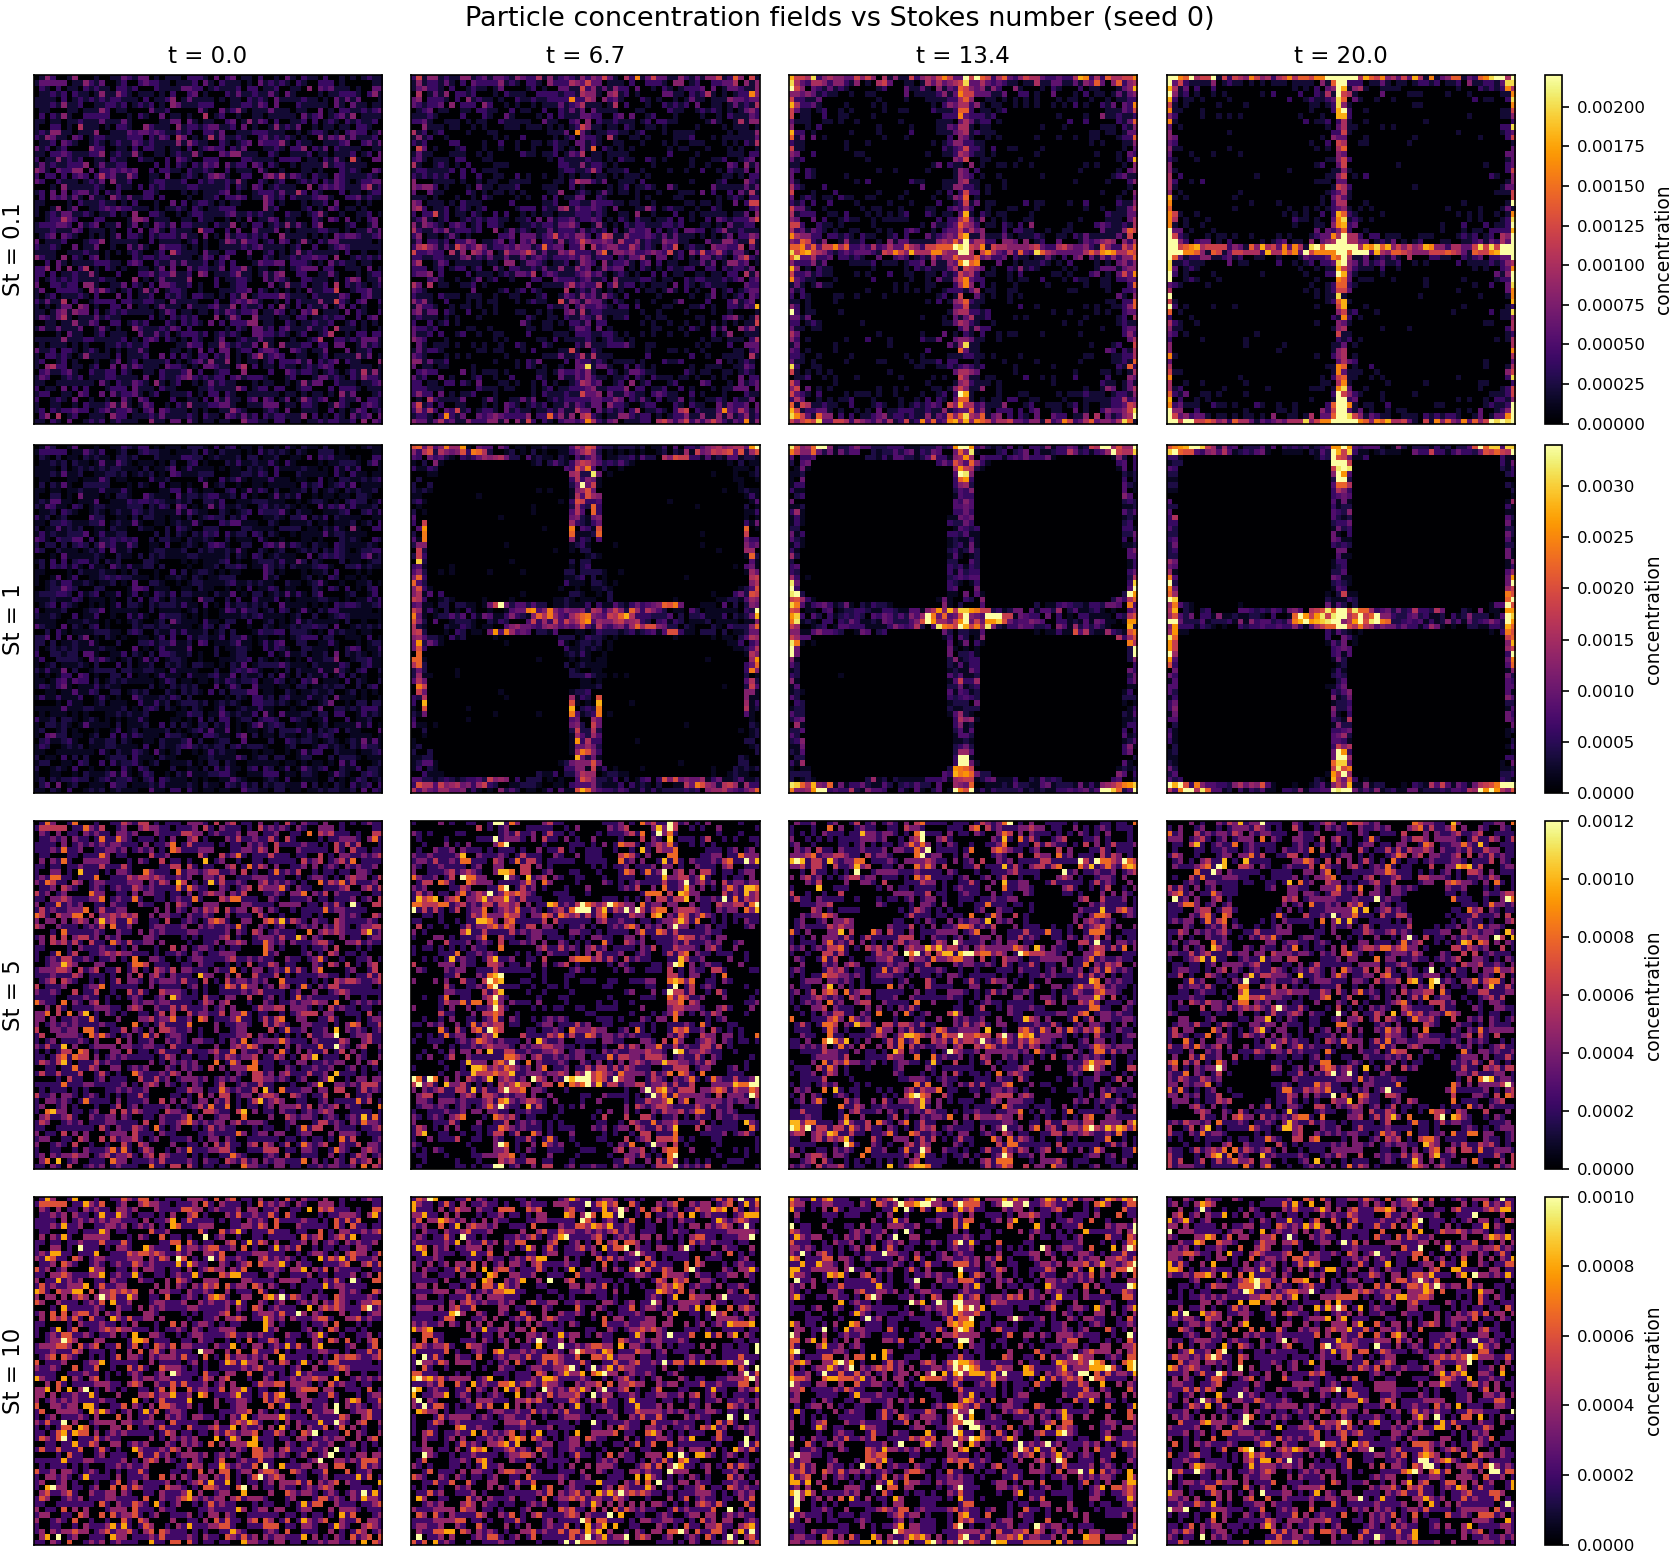
\includegraphics[width=\columnwidth]{stokes_comparison.png}
  \caption{% TODO
  Concentration fields versus Stokes number and time.}
  \label{fig:stokes}
\end{figure}

\section{Reduced-Order Representation}
% POD and the convolutional autoencoder at equal latent size; the shot-noise
% floor on raw fields; what changes on the smoothed fields and on the Fourier
% flow.

\begin{table}[t]
  \centering
  \caption{% TODO
  Reconstruction error at latent dimension 16.}
  \label{tab:reconstruction}
  \begin{tabular}{lccc}
    \toprule
    Dataset & POD & Autoencoder & Modes for 90\,\% energy \\
    \midrule
    Raw    &  &  &  \\
    Smooth &  &  &  \\
    Fourier &  &  &  \\
    \bottomrule
  \end{tabular}
\end{table}

\section{Latent-Space Forecasting}
% The recursive roll-out protocol; persistence baseline; DMD as the linear
% latent map; the neural forecasters (MLP, Neural-ODE, GRU) and the roll-out
% curriculum.

\begin{figure}[t]
  \centering
  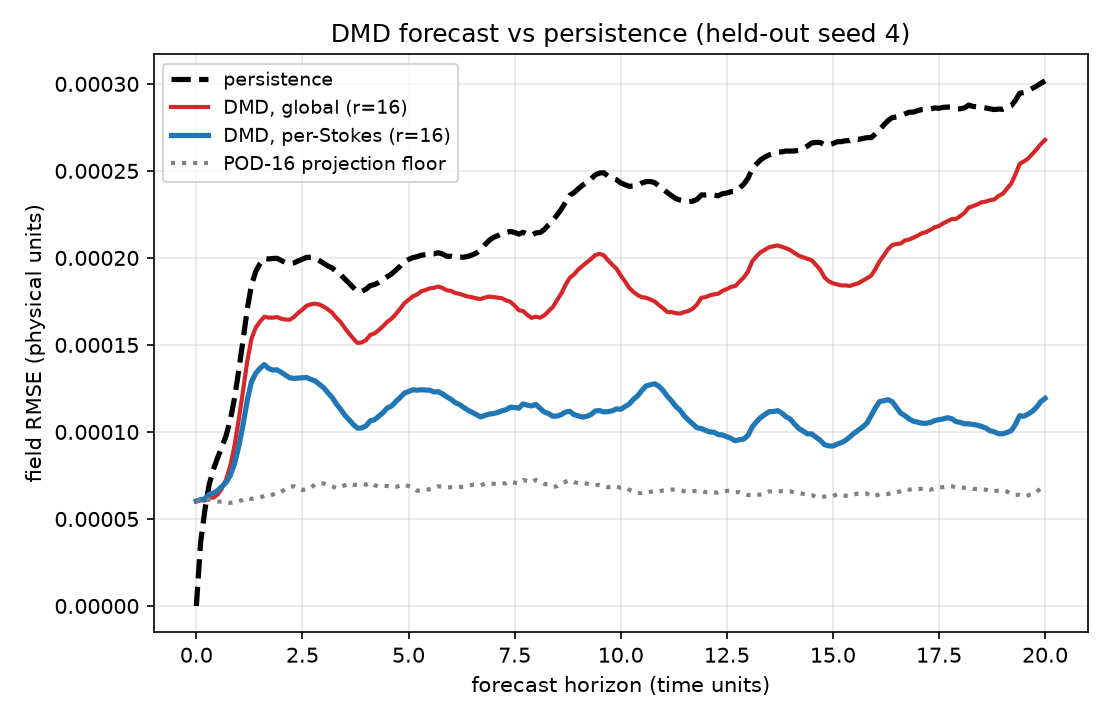
\includegraphics[width=\columnwidth]{dmd_forecast_smooth.png}
  \caption{% TODO
  DMD forecast against persistence on the held-out seed.}
  \label{fig:dmd}
\end{figure}

\section{Results}
% Seed-averaged comparison at fixed horizons; where the neural models win
% (short horizons) and where DMD wins (long horizons); the reproducibility
% check.

\section{Limitations}
% Prescribed laminar flow, one-way coupling, the shot-noise floor, and the
% seed sensitivity of the neural forecasters.

\section{Conclusions}
% What a reader should take away, in three or four sentences.

% Uncomment both lines once refs.bib holds at least one entry you \cite:
%\bibliographystyle{IEEEtran}
%\bibliography{refs}

\end{document}
